Un knowledge graph (KG ou graphe de connaissance ou réseau de connaissance) est défini comme une base de connaissance organisé sous forme de graphe \cite{ehrlinger2016towards} \cite{JoStichburyKG}. Comme pour une base de connaissance, l'information est organisée à l'aide d'ontologies. De part l'intégration d'une sémantique de l'information, il est possible de dériver du savoir de l'information disponible. 

Modéliser notre problème de fact checking sous la forme d'un graphe va nous permettre d'utiliser des propriétés et comportement définis dans la théorie des graphes. Les graphes vont nous permettre de comprendre un fait en analysant leur environnement. Cela va nous permettre de fournir ce qui manque à d'autres systèmes de fact checking comme ClaimBuster : un contexte sémantique. Il va complémentariser certaines approches utilisant le machine learning ou encore des approches qui se basent sur le TAL en leur apportant une image de l'existant, un environnement plus vaste. Un KG va permettre d'avoir un aperçu factuel et précis de l'existant. Il va nous apporter un système qui va se baser sur les relations entre les entités définies dans le fait et les confronter avec celles dans l'existant pour établir un verdict. 
Nous commencerons par voir une application basique, la plus simple possible, d'une approche de fact checking à base de KG. Puis nous verrons des méthodes qui étendent et améliorent cette approche.

\subsection{Wikipédia knowledge graph}

Le travail suivant repose sur les recherches effectuées ici \cite{ciampaglia2015computational}. Nous tâcherons d'analyser et comprendre le travail effectué, ensuite nous évaluerons sa faisabilité de son couplage avec d'autres modules qui permettront de renforcer et améliorer la fiabilité d'un système de fact checking. Suite aux recherches effectuées dans ce papier il a été prouvé qu'utiliser un graphe non orienté avec l'approche présentée ci-dessous est la plus optimale.

Pour commencer notre démonstration nous allons partir d'une assertion simple : dans un graphe une entité est liée à une autre entité s'il existe un chemin ne dépassant pas  x entités d'écart. Soit un fait en rapport avec deux entités, si ces deux entités ne sont pas liées ou si une des deux entités n'est pas présente dans le graphe, alors il y a de fortes chances pour que ce fait soit faux. Pour rappel, comme pour une base de connaissance, dans un graphe de connaissance l'information est organisée sous la forme de triplet <Sujet, Prédicat, Objet>. Entre deux entités on peut avoir plusieurs chemins de longueurs variables. Chaque chemin apporte des informations distinctes et plus ou moins précises sur la relation entre ces entités. Rechercher le chemin le plus court possible entre deux entités va nous permettre d'établir un lien de véracité sur lequel nous allons nous baser pour déterminer si un fait est vrai ou faux.
\\*
Par exemple pour l'assertion suivante : \enquote{Joseph Boyden wrote Three Day Road} on a 2 entités, l'écrivain et l'ouvrage. Pour arriver de l'un à l'autre on va avoir des chemins directs : l'objet livre va avoir une relation de type \enquote{auteur} qui va directement lier le livre et son auteur. On va donc attribuer une valeur forte à cette relation. Un autre chemin qui passera par des entités plus génériques se verra attribuer une importance plus faible. La recherche du chemin le plus court se résume à la recherche du chemin qui a le plus de sens dans ce contexte.

Dans cette approche il est important de bien définir l'impact et le rôle de la longueur du chemin entre deux entités. 
Soit G un graphe non orienté et G = (V, E) où V représente nos sommets, nos entités et E les relations entre ces entités. Pour déterminer l'existence d'un lien entre deux entités on va utiliser une opération mathématique dite \enquote{Fermeture transitive}. Le calcul de la fermeture transitive va nous permettre de créer un graphe annexe où toutes les relations sont déjà déterminées (pré-traitement qui va nous permettre de trouver plus facilement s'il existe un lien entre 2 entités) \cite{JJLGraphes}.

\begin{figure}[H]
  \centering
  \begin{minipage}[b]{0.4\textwidth}
    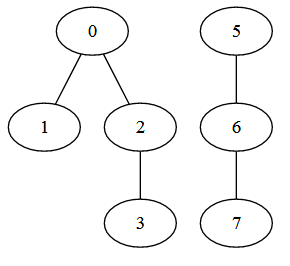
\includegraphics[width=\textwidth]{imgs/graph.PNG}
    \caption{Graphe original, non orienté}
  \end{minipage}
  \hfill
  \begin{minipage}[b]{0.4\textwidth}
    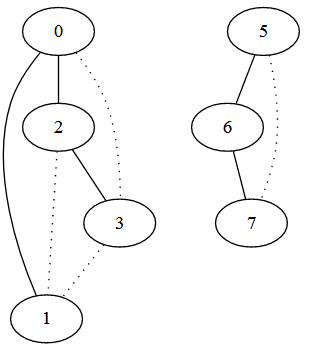
\includegraphics[width=\textwidth]{imgs/graphFT.PNG}
    \caption{Graphe et sa fermeture transitive}
  \end{minipage}
\end{figure}

\iffalse
Code du graphe (enlever les dotted pour le graphe original)

graph G {
	0 -- 1
    0 -- 2
    2 -- 3
    5 -- 6
    6 -- 7
    3 -- 1 [style=dotted]
    5 -- 7 [style=dotted]
    2 -- 1 [style=dotted]
    0 -- 3 [style=dotted]
}
\fi

On va attribuer à chaque chemin une valeur de confiance ou score de confiance qui va déterminer si ce chemin peut être utilisé pour évaluer un fait. Ce score va d'abord dépendre du degré (liens avec d'autres entités) des noeuds traversés. Une entité générique aura un degré important ce qui diminuera le score de confiance, ex : un pays, une grande organisation, etc. D'un autre côté ce score sera plus élevé s'il traverse des noeuds moins génériques, ex : personne, livre, etc. En effet un lien entre deux entités sera plus pertinent si le chemin ne traverse que des entités avec peu de relations et le contexte sémantique sera plus précis. En suivant la même logique lorsque deux entités sont directement liées, on va leur accorder un score de confiance maximal : il n'y a pas d'intermédiaires.

Le chemin qui aura le score le plus élevé sera le chemin le plus court et qui traversera les entités les moins générique. C'est ce que l'on va appeler la proximité sémantique. Cette proximité sémantique représente le sens qui relie deux entités. Pour un fait donné, est-ce que c'est deux entités mise bout à bout ont du sens ? 

Pour le moment nous avons vu comment choisir un chemin entre deux entités, qui va nous permettre ensuite de déterminer si un fait est vrai ou faux. 
\\*
Pour illustrer ceci, prenons un exemple, soit des faits qui lient des villes avec des pays. Pour chaque pays et chaque villes on va tester l'assertion : \enquote{La capitale du pays x est y}.

\begin{figure}[h]
\centering
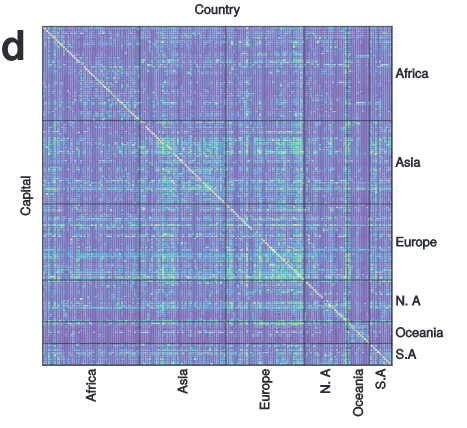
\includegraphics[draft=false, scale=0.5]{imgs/country_cap_check.PNG}
\caption{Pays et capitales groupées par continent}
\label{fig1}
\end{figure}

\todo{\url{http://www.kurzweilai.net/a-computational-algorithm-for-fact-checking}}

Plus un point est clair et plus le fait a de chance d'être vrai. Le chemin entre un pays et sa capitale possède une proximité sémantique plus forte que le chemin entre un pays et n'importe quelle autre ville. Bien que cette méthode soit très basique, elle apporte des résultats satisfaisant. Le taux de réussite selon les datasets utilisés varie entre 61\% et 95\%. Cet exemple prouve que le fact checking peut se faire au travers de graphes de connaissances. 

\paragraph{Critique} Cette méthode permet de faire du fact checking sur des faits simples. Elle se fait entre deux entités clairement définies. Le champs des possibles pour les faits à vérifier est donc limité.

Problème de scalabilité, important d'avoir le verdict instantanément.

Nous verrons plus tard, avec des méthodes plus avancées, certains problèmes inhérents à l'utilisation de KG pour le fact checking.

Ciampaglia et al. [8] propose
an approach that relies on a single short, specific path to
differentiate a true fact from a false one. Although intuitive,
their algorithm fails to account for the semantics of the target
predicate

\todo{Ouvrir sur la seconde approche knowledge stream et montrer qu'il améliore cette approche}

\todo{A lire : https://searchengineland.com/google-researchers-introduce-system-rank-web-pages-facts-not-links-215835}
\label{sec:wkg}

\subsection{Fact checking à base de réseaux de flots} 

Nous avons vu que le fact checking de faits simples était possible via le parcours d'un graphe de connaissance. Seulement plusieurs problèmes peuvent se poser comme la montée en charge d'une telle approche ou sa fiabilité. Dans ce papier, une nouvelle approche est utilisée pour organiser et parcourir un graphe de connaissance. Le code source est disponible \href{https://github.com/shiralkarprashant/knowledgestream}{ici}.

\begin{wrapfigure}{r}{0.5\textwidth}
  \begin{center}
    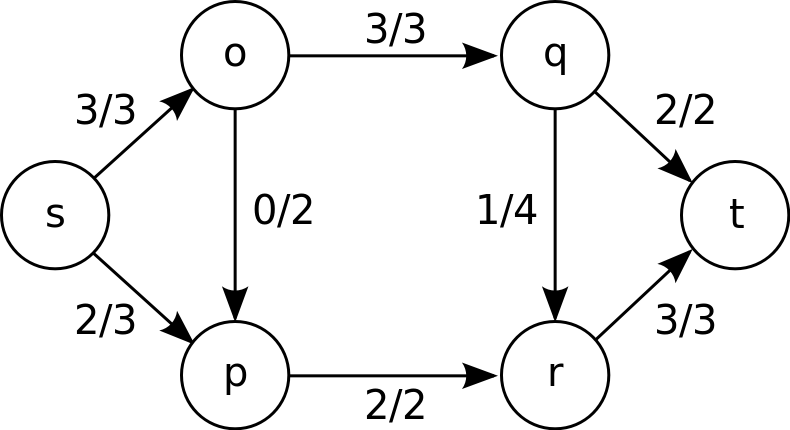
\includegraphics[width=0.6\textwidth]{imgs/max_flow.png}
  \end{center}
  \caption{Graphe/Réseau de flot non orienté}
  \label{max_flow}
\end{wrapfigure}

Cette approche consiste à organiser un graphe comme un réseau de flot \cite{shiralkar2017finding}. Dans un réseau de flot, chaque arête possède une capacité maximale dans laquelle peut passer un flux. Avec cette approche on va chercher à évaluer sémantiquement chaque chemin allant d'une entité A vers une entité B. Plusieurs chemins vont apporter plusieurs contextes qui vont permettre d'évaluer sémantiquement le fait. En outre, la recherche de chemins optimaux est limité par la capacité maximale de chaque arête. 
\\*
En travaillant sur un réseau de flot et en contraignant ainsi chaque flux, on réduit le nombre de chemins possibles entre deux entités. De plus on limite le nombre d'arêtes communes entre chaque chemin. On a ainsi des chemins plus variés en terme de contexte sémantique. Dans la figure \ref{max_flow}, pour aller de s vers t il est possible de passer par l'arête p \textrightarrow r, sans contraintes, l'algorithme passera toujours par cette arête. L'espace restreint va l'obliger à passer par o \textrightarrow q et ainsi fournir de nouvelles informations.
\\*
Ces chemins vont construire l'argumentaire sur lequel le système va s'appuyer pour rendre un verdict sur le statut d'un fait.

\begin{figure}[H]
\centering
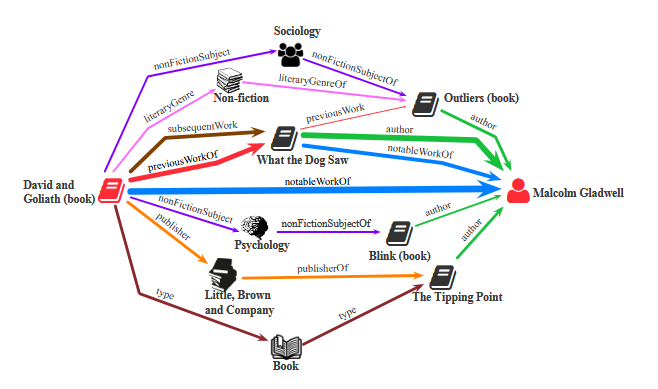
\includegraphics[width=\textwidth, draft=false]{imgs/bookAuthorKG.PNG}
\caption{Relations entre un livre et son auteur dans un graphe de connaissance \cite{shiralkar2017finding}}
\label{stream}
\end{figure}

La figure \ref{stream} représente l'argumentaire autour du triplet t = (David and Goliath (book), author, Malcolm Gladwell). Plus une arête est directe et plus elle est épaisse. Plus elle est épaisse et plus le flux d'informations est important. Cela permet de privilégier les chemins courts dans lesquels les informations contenues sont sémantiquement importantes. 
\\*
Pour un triple donné (s, p, o) il faut voir l'information comme une quantité abstraite qui doit voyager du sujet s vers l'objet o. Chaque arête possède une capacité permettant de transporter plus ou moins d'informations, mais aussi un coût d'utilisation. Ce coût d'utilisation représente le coût d'envoi d'une unité d'information sur le réseau. Ce coût d'utilisation permet encore de s'assurer que les chemins seront le plus court et spécifique possible.
\\*
Le but est donc de trouver les chemins pour lesquelles nous pouvons transporter le plus d'informations entre s et o pour un coût minimal.

\paragraph{Fact checking dans un réseau de flot}

Nous allons voir à présent deux méthodes de fact checking qui appliquent ce concept de réseau de flot dans un graphe de connaissance : Knowledge Stream et Relational Knowledge Linker. Ces méthodes vont construire l'argumentaire d'un fait autour des relations entre les triples qui composent un chemin.

\subsubsection{Knowledge Stream}
\label{sec:ks}

\paragraph{Analogie entre les relations}

Afin de construire un contexte qui va être le plus proche possible de celui du fait énoncé, on va déterminer les relations homologues entre celle du fait et celles existantes dans notre KG. Par exemple pour déterminer l'auteur d'un livre on ne va pas aller regarder les relations concernant l'architecture mais bien celles concernant la littérature.

Pour évaluer l'analogie entre les relations on va construire un graphe G dans lequel les sommets sont des entités et les arêtes des relations. Dans la figure \ref{graph_g},  entre les entités A et C on a une relation de type c (qui peut être par exemple une relation de type \enquote{est marié à}).
\\*
La figure \ref{linear_g_graph} représente le graphe adjoint de G. Par définition, étant donné un graphe G non orienté, le graphe adjoint de G, noté L(G), est un graphe qui représente la relation d'adjacence entre les arêtes de G. Ainsi chaque sommet de L(G) représente une arête de G. Deux sommets de L(G) sont adjacents si et seulement si les arêtes correspondantes partagent une extrémité commune dans G \cite{wiki:lg}.
\\* 
Dans la figure \ref{linear_g_graph} on peut voir que certains noeuds sont représentés plusieurs fois comme a1 et a2 alors qu'ils définissent la même relation. Pour palier à ce problème il faut contracter le graphe comme dans la figure \ref{w_line_graph}. On fusionne chaque sommet commun et on pondère les arêtes en fonction des relations précédentes des sommets.
\\*
Cette démarche va nous permettre de définir les similarités entre les relations. Les arêtes pondérées dans la figure \ref{w_line_graph} représentent la fréquence à laquelle chaque relation co-incident avec ses voisins dans G. Plus cette pondération est importante et plus la similarité entre les relations est forte.

Au final, à partir de la matrice d'adjacence du graphe contracté, on va pouvoir établir des corrélations entre les différentes relations (ici les sommets) à l'aide du TF-IDF (term frequency-inverse document frequency). Cette méthode va évaluer l'importance d'une relation au sein du graphe. Déterminer l'importance d'une relation va nous permettre d'établir un contexte plus précis pour un fait donné. 

\iffalse
Code du graphe G original

graph G {
    A -- B  [label="a1"];
    A -- C  [label="c"];
    A -- D  [label="a2"];
    B -- C  [label="b"];
    C -- E  [label="e1"];
    C -- F  [label="f"];
    D -- E  [label="d"];
    E -- F  [label="e2"];
}

G linear graph

graph G {
    a1 -- a2
    a1 -- c
    a1 -- b
    a2 -- d
    a2 -- c
    b -- c
    b -- e1
    b -- f
    c -- e1
    c -- f
    d -- e1
    d -- e2
    e1 -- e2
    e1 -- f
    e2 -- f
}

Weighted G linear graph

graph G {
    a -- b [label="1"];
    a -- c [label="2"];
    a -- d [label="1"];
    b -- c [label="1"];
    b -- e [label="1"];
    b -- f [label="1"];
    c -- e [label="1"];
    c -- f [label="1"];
    d -- e [label="2"];
    e -- f [label="2"];
}
\fi

\begin{figure}[H]
  \centering
  \begin{minipage}[b]{0.3\textwidth}
    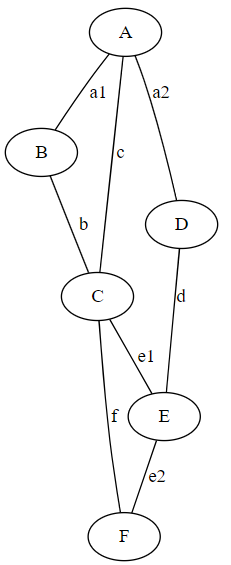
\includegraphics[width=\textwidth]{imgs/graph_g.PNG}
    \caption{Graphe G original, non orienté}
    \label{graph_g}
  \end{minipage}
  \hfill
  \begin{minipage}[b]{0.3\textwidth}
    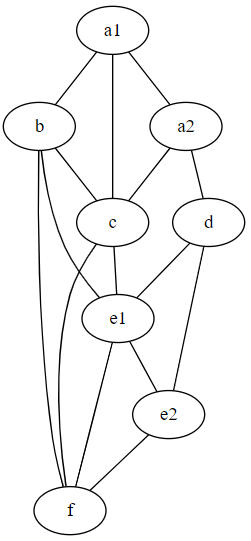
\includegraphics[width=\textwidth]{imgs/linear_g_graph.PNG}
    \caption{Graphe adjoint G'}
    \label{linear_g_graph}
  \end{minipage}
  \hfill
  \begin{minipage}[b]{0.3\textwidth}
    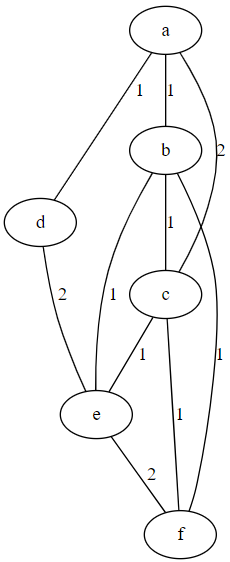
\includegraphics[width=\textwidth]{imgs/w_line_graph.PNG}
    \caption{Graphe adjoint contracté G*}
    \label{w_line_graph}
  \end{minipage}
\end{figure}

\paragraph{Problème de minimisation dans un réseau de flot}

Pour rappel nous cherchons à trouver l'ensemble des chemins pour lesquels le flux maximum est poussé de s vers o pour un coût minimal. Un réseau de flot vient avec différentes contraintes. Il faut tout d'abord pouvoir déterminer la pondération des relations entre les entités, savoir combien d'unités d'information je peux passer d'une entité à une autre. Pour cela on va se baser sur le calcul précédent qui détermine la similarité entre les relations. La quantité disponible pour chaque flux sera calculé selon la similarité avec le prédicat du triplet cible. Plus deux relations seront similaires et plus le flux alloué sera important. En outre, plus un fait sera général (plus il aura de relations), moins son flux sera important.

Une autre contrainte énoncée plus haut est le coût d'utilisation du réseau, chaque chemin à un coût. On cherche à minimiser ce coût et dans cette approche minimiser le coût signifie traverser le moins d'entités génériques possible. Les entités trop génériques ne permettent pas de récupérer des informations précises dans un contexte donné. Le coût d'utilisation d'une arête sera donc déterminé par les relations de ses sommets avec les sommets adjacents.

La dernière contrainte est que dans un réseau de flot, le flux entrant dans un sommet doit être égal à son flux sortant. Il faut pouvoir déterminer le flot maximum qui peut être envoyé entre s et o.
\\*
Cette contrainte est représentée ainsi :
\begin{equation}
   \sum\limits_{P_{s,p,o}  \in  \mathcal{P}_{s,p,o}}  \beta(P_{s,p,o})
\end{equation}

Où $ \beta(P s,p,o) $ représente le plus petit flot possible pour un chemin. Il s'agit de l'arête qui possède la capacité minimale sur un chemin. Les unités d'informations que je peux envoyer sur un chemin seront limitées par $ \beta(P s,p,o) $. Dans cette approche, cette arête représente le triple le moins pertinent pour notre chemin.
\\*
Si on reprend la figure \ref{max_flow}, on ne pourra jamais envoyer plus de 5 unités d'informations de s vers t. En effet les chemins qui mènent vers t sont limités. Si entre o et q mon flot maximum était de 2, alors je ne pourrais jamais envoyer plus de 4 unités d'informations de s vers t. Donc l'information maximale que je peux envoyer se calcul à partir de la somme des capacités minimales de chaque chemins allant de s vers t. Soit la somme des $ \beta(P s,p,o) $.

Au final, sachant que je peux envoyer x unités d'information sur mon réseau, comment maximiser les informations viables que je peux récupérer ? Pour cela il faut pouvoir déterminer des chemins spécifiques pour éviter les chemins trop génériques. Ex : si mon chemin passe par l'entité \enquote{France} on va lui attribuer une faible valeur sémantique. On solutionne ce problème par la contrainte suivante :

\begin{equation}
   \mathcal{S}(P_{s,p,o}) = \frac{1}{1 + \sum\limits_{i=2}^{n-1} \log k(v_{i})}
\end{equation}

Où $ k(v_{i}) $ représente le degré du noeud $ v_{i} $. On va établir un score sémantique déterminé par la somme des degrés des noeuds (nombre de relations) en relation avec $ P_{s,p,o} $. Plus $ P_{s,p,o} $ aura de relations et plus il aura de relations génériques, moins son score sémantique sera élevé.

Ainsi nous allons pouvoir établir un score de fiabilité pour un triple :
\begin{equation}
   \beta(P_{s,p,o}) \times \mathcal{S}(P_{s,p,o})
\end{equation}

Pour un triple donné, son score de fiabilité sera évalué par le produit entre le flot maximum que peut porter le chemin et le score sémantique du triple. Pour rappel, plus un triple est direct et plus son flot maximum est élevé. Un triple avec un score élevé sera court, le plus direct possible, et aura peu de relations avec des entités génériques. Finalement, pour évaluer le score de fiabilité d'un chemin, il suffit de sommer tous les scores de fiabilité des triples qui le compose.

\subsubsection{Relational Knowledge Linker}

Cette approche cherche à étendre des méthodes de fact checking sur des graphes de connaissance déjà existants.
Pour l'approche précédente on se concentre sur la sémantique du sujet et de l'objet, on favorise le sens que l'on peut tirer du triple. L'argumentaire se construit autour de la spécificité de chaque triple.
\\*
Dans cette approche on va se concentrer sur la similarité entre les relations qui lient l'objet et le sujet pour construire notre argumentaire. On se base sur la sémantique du prédicat. Ainsi on va chercher à maximiser la sémantique autour des relations entre les triples. Cette approche étend ce que nous avons vu dans la section \ref{sec:wkg} en y ajoutant la similarité entre les relations.

\subsubsection{Critique}

L'évaluation de cette approche s'est faite sur des datasets déjà formatés, des triples issus notamment du Google Relation Extraction Corpora
(disponible \href{https://github.com/google-research-datasets/relation-extraction-corpus}{ici}). Aucune application dans la vie réelle n'a été conduite. Pour des cas d'application réels il faut pouvoir vérifier un fait en langage naturel. Pour cela il faut pouvoir identifier dans un fait, et avec certitude, les deux entités et la relation qui les unit. On en revient à un problème de TALN. Comment je vais fournir à mon système des données qu'il peut traiter ? On peut envisager plusieurs méthodes pour palier à ce problème, les faits devant être simples, on peut utiliser le TALN ou le machine learning \cite{googleai}. On ne peut pas simplement analyser chaque mot et le comparer avec les données présentes dans le graphe. C'est possible pour identifier les entités, mais pour ce qui est des relations il y a toujours plusieurs façons d'exprimer un même lien.

Pour rappel, cette approche permet de faire du fact checking sur des faits de la forme d'un triplet. Soit des faits simples. Et bien que les faits soient simples, le temps pour vérifier un seul fait se calcul selon une complexité pseudo-polynomiale. Soit $ O(Y|E|\log |V|)$ où V représente les sommets du graphe, E les arêtes et Y le flot maximum d'informations que l'on peut faire passer sur le réseau. Sur des graphes géants tels que DBPedia on obtient un temps moyen (sur laptop) de 356 secondes pour la vérification d'un fait. On peut s'interroger sur l'utilité d'une telle approche pour vérifier des faits en live ou même pour servir d'outil pour aider les journalistes. Avec cette approche la complexité va grandissante en fonction de la taille du graphe. Travailler sur des graphes complets, qui bénéficient de grandes quantités d'informations peut demander beaucoup de temps. Le graphe utilisé pour conduire les expériences est issu des infobox de wikipédia et est constitué de 6 millions d'entités donnant 24 millions de triples déterminés par 663 relations différentes. En comparaison, wikidata est constitué de plus de 48 millions d'entités \cite{wikidata:statistics} \cite{wikidata:statistics2} et le Google Knowledge Graph de plus de 500 millions d'entités et 3.5 milliards de faits à leur sujet \cite{google:kg}.

Pour une montée en charge il faut pouvoir réduire ce temps de calcul. Pour cela il faudrait pouvoir abroger ou du moins anticiper le caractère unique de chaque fait. En effet, pour un fait a traiter, il faut reproduire toutes les étapes vues précédemment. Il est impossible de réutiliser des données calculées en amont, sur d'autres faits, pour réduire le temps de calcul. En effet, pour chaque fait le graphe se modélise de façon unique. Pour chaque fait les entités et relations en cause ne seront pas les mêmes. Il est donc nécessaire de reconstruire le graphe.

Une autre limitation est la rareté de la donnée. Bien que les bases de connaissances existantes soient immenses, elles ne sont pas comparables au flux de données quotidien qui transite sur internet. De plus les bases de connaissances comme Wikidata ou DBPedia ne contiennent aucune news ou informations récentes. Pour DBPedia on ne pourra vérifier un fait que si l'information est présente dans wikipédia. D'autre part, si ce manque de données venait à être résolu on se retrouverait avec des graphes tellement grands qu'il serait impossible de les analyser dans des temps raisonnables avec les méthodes présentées.


\subsection{Conclusion}

Nous avons vu que les KG permettent de réaliser des opérations de fact checking sur des faits simples dans des temps plus ou moins raisonnables. Du fait du manque de données et de la complexité des faits à analyser il est difficile de penser à un système de fact checking entièrement autonome à base de KG. Le temps de calcul est aussi un frein important. En revanche cette approche nous apporte des informations essentielles pour les autres méthodes et système de fact checking : un contexte sémantique. Ce contexte sémantique se matérialise par la construction de l'argumentaire d'un fait qui évalue son environnement et confronte ses liens avec l'existant. Pour ClaimBuster par exemple cela permettrait d'ajouter du sens à l'information et ainsi améliorer sa recherche d'information permettant de contextualiser le fait.

D'autres part il est possible d'étendre cette approche vers des modèles de statistiques prédictives pour palier à ce manque de scalabilité \cite{wilcke2017knowledge}. C'est-à-dire analyser des faits présents et passés pour faire des hypothèses sur des événements futurs. Appliqué au machine learning il serait possible d'entraîner le système au fil des requêtes pour améliorer le temps de construction du graphe associé aux similarités entre les relations et appliquer un verdict sur un fait plus rapidement. Il est aussi possible de construire un argumentaire qui s'étendrait sur plusieurs faits, c'est-à-dire traiter un fait comme étant en relation avec d'autres faits. Ainsi il serait possible de construire une cohérence dans un texte entre les faits analysés.

Pour réaliser une approche par les graphes de connaissances il est possible de faire appelle à des apis, notamment celle du Google Knowledge Graph (GKG) ou Unigraph. Le GKG est ce qui permet au moteur de recherche de Google d'ajouter de la sémantique aux résultats d'une requête. Il est possible pour des faits simples et corrélés de trouver un lien déterminant pour assurer un verdict. Par exemple, il est possible de résumer la méthode précédente à une simple requête et à l'analyse syntaxique de la réponse. Si on prend l'assertion suivante : \enquote{Joseph Boyden wrote Three Day Road}. Si on recherche sur l'api les deux entités, on va tout de suite établir le lien entre elles. En annexe sont disponibles les fragments important retournés par l'api (\ref{appendix:gkg_jb}). 

Enfin, les KGs sont importants pour les modèles qui se reposent sur le machine learning. Ils apportent de la donnée structurée, contextualisée et compréhensible pour la machine. Aujourd'hui, les algorithmes de type machine learning sont entraînés avec de la donnée la plus pure et brute possible. Fournir à ces algorithmes des données plus sophistiquées pourrait permettre de construire des systèmes plus intelligents \cite{nickel2016review}. Cela permettrait en outre de réduire les temps de travail nécessaires pour chaque requêtes.

Certains systèmes implémentent déjà une approche par les KG avec le TAL pour le traitement des données, ex \cite{gerber2015}. 